\section{Classification of covariance matrices for SSVEP}
\label{sec:classofcov}

\iflatexml\else \changes{ \fi

\subsection{Fundamentals of classification}
\label{subsec:fund_class}

Given labelled samples $\x_i$ drawn from two classes or populations (positive and negative), a simple classification algorithm consists in assigning a previously unseen sample to the class with closer mean[ref: fig].
This implies a computation of means of class and a measure of distances from the means. 
Assuming that the samples are embedded into a dot product space (i.e. with Euclidean geometry), the means can be computed as:

\begin{equation}
c_{+} = \frac{1}{m_{+}} \sum_{ \left\lbrace i|y_i=+1 \right\rbrace } \x_i,
\label{eq:mean_eucl1}
\end{equation}

\begin{equation}
c_{-} = \frac{1}{m_{-}} \sum_{ \left\lbrace i|y_i=-1 \right\rbrace } \x_i,
\label{eq:mean_eucl2}
\end{equation}
where $y_i \in \left\lbrace +1, -1 \right\rbrace$ is the label of the training sample $\x_i$, $m_{+}$ and $m_{-}$ the number of positive and negative samples respectively. 
An unseen sample $\x$ is unsigned to the class whose mean is the closest. 
This simple geometric classification framework is the founding principle of more complex algorithms such as supporting vector machines. 
\iflatexml\else } \fi

\iflatexml\else \changes{ \fi
It can be formulated in terms of the dot product $\left\langle \cdot, \cdot \right\rangle$.
If $c:=(c_{+}+c_{-})/2$ is the point lying halfway between $c_{+}$ and $c_{-}$, and $w:=c_{+}-c_{-}$ the vector connecting $c_{+}$ to $c_{-}$, the class $y$ of the unseen sample $\x$ is determined by checking whether the vector $\x-c$ connecting $c$ to $x$ makes an angle $\alpha < \pi/2$ with $w$ [ref: fig].   
This is expressed as:

\begin{equation}
\begin{split}
y &= \mathrm{sgn} \left\langle (\x-c),w \right\rangle \\
  &= \mathrm{sgn} \left\langle (\x-(c_{+}+c_{-})/2),(c_{+}-c_{-}) \right\rangle \\
  &= \mathrm{sgn} (\left\langle \x,c_{+} \right\rangle - \left\langle \x,c_{-} \right\rangle + b)
\end{split}
\label{eq:classif1}
\end{equation}
where $\mathrm{sgn}$ is the sign function.
The offset $b$ vanishes if class means are equidistant to the origin \cite{scholkopf_learning_2001}.
Inserting \eqref{eq:mean_eucl1} and \eqref{eq:mean_eucl2} in \eqref{eq:classif1} yields:

\begin{equation}
y = \mathrm{sgn} \left( \frac{1}{m_{+}} \sum_{ \left\lbrace i|y_i=+1 \right\rbrace } \left\langle \x,x_i \right\rangle - \frac{1}{m_{-}} \sum_{ \left\lbrace i|y_i=-1 \right\rbrace } \left\langle \x,\x_i \right\rangle + b \right) .
\label{eq:classif2}
\end{equation}
Classifier \eqref{eq:classif2} can be generalized as:

\begin{equation}
y = \mathrm{sgn} \left( \sum_{i=1}^{m} y_i \alpha_i \dist(\x,\x_i) + b \right) ,
\label{eq:classif_gen}
\end{equation}
where $\alpha_i$ is the weight of the training sample $x_i$ and $\dist(\cdot, \cdot)$ a distance, a divergence of a kernel. 
In the case of two classes, with $m$ samples ($m = m_{+} + m_{-}$) in the dot product space where all samples have the same weight, $y_i \in \left\lbrace +1, -1 \right\rbrace$, $\alpha_i = 1/m$ and $\dist(\cdot, \cdot) = \left\langle \cdot, \cdot \right\rangle$. 
\iflatexml\else } \fi

\iflatexml\else \changes{ \fi
Expression~\eqref{eq:classif_gen} corresponds to the decision function used in hyperplane classifiers \cite{scholkopf_learning_2001}. 
This shows that even more complex classifiers rely on the calculations of class means (or centers) and their distances to individual samples.
This being shown, in this article we focus on the simple classification approach of assigning a previously unseen sample to the class with closest mean.
\iflatexml\else } \fi

\iflatexml\else \changes{ \fi
In machine learning algorithms, samples are represented by their features which are determined through a feature extraction and selection process.
In this work, samples are represented by their covariance matrices. Therefore means of classes and distances to mean will be means of covariance matrices and distance between them.
\iflatexml\else } \fi

\subsection{Means of Covariance matrices}
\label{subsec:mean}

\iflatexml\else \changes{ \fi
Consider a multivariate variable $\X \in \Re^{\dc \times \dt}$ where $\dc$ is the number of variables and $\dt$ the number of samples, with $C > N $, the covariance matrix of the centered variable $\X$ can be estimated as:

\begin{equation}
\P = \frac{1}{\dt} \X \X^\intercal
\end{equation}
and is symmetric positive definite (SPD): $\P \in \Ma$, a manifold of $\dc\times\dc$ symmetric positive definite matrices,
\begin{equation*}
	\label{eq:rm}
  \Ma = \left\{ \P \in  \Re^{\dc\times\dc} : \P = \P^\intercal \text{ and } x^\intercal \P x > 0, \forall x \in \Re^{\dc} \backslash 0 \right\} \ . %\nonumber
\end{equation*}
The properties of SPD matrices constrain them to a convex cone:

\begin{enumerate}
[label=(\roman*)]
\item Symmetry: \tab $\P = \P^\intercal$ ,
\item Positive definiteness: \tab $\x^\intercal \P \x > 0, \forall x \in \Re^{\dc} \backslash 0$ ,
\item Strict positivity of diagonal element: \tab $\P(i,j) > 0 | i=j, \forall i,j \in \left\lbrace 1, \dots, \dc \right\rbrace$ i.e. positive variance ,
\item Cauchy-Schwarz inequalities: \tab $|\P(i,j)| \leq (\P(i,i) \P(j,j))^{1/2}, \forall i,j \in \left\lbrace 1, \dots, \dc \right\rbrace$ .
\end{enumerate}
\iflatexml\else } \fi

\iflatexml\else \changes{ \fi
The mean of SPD matrices can be computed as a center of mass modeled on Euclidean geometry:}
given a set of covariance matrices $\{\P_\nb\}_{\nb=1,\dots,\Nb}$,
the center of mass $\Pm$ of the set, is a covariance matrix that minimizes the sum of the squared distances to matrices $\P_\nb$:

\begin{equation}
	\label{eq:mean}
	\Pm = \Rm(\P_1, \dots, \P_\Nb) = \argmin_{\P \in \Ma} \sum_{\nb=1}^{\Nb} \dist^2(\P_\nb,\P) \ ,
\end{equation}
where $\dist(\cdot,\cdot)$ is a measure of distance between two matrices. 
\iflatexml\else \changes{ \fi
Practically, $\dist(\cdot,\cdot)$ can either be a distance or a divergence.
\iflatexml\else } \fi
\iflatexml\else \changes{ \fi
In the literature, this  mean is at times designated as the \emph{Frechet mean}, \emph{Cartan mean}, or \emph{Karcher mean} \footnote{This appellation has been recently criticized by Karcher himself \cite{karcher_riemannian_2014}} \cite{lim_matrix_2012}.
Cartan \cite{cartan_groupes_1929} had shown that a unique solution to \eqref{eq:mean} exists if all $\P_\nb$ lie in a convex ball \citep[section 16 of][]{cartan_groupes_1929}. This applies also to closed convex cones.
\iflatexml\else } \fi

\iflatexml\else \changes{ \fi
Depending on the divergence or distance used, several means can be defined from \eqref{eq:mean}. Those considered in this study are presented in the next lines and summarized in Table~\ref{tab:dist}.
\iflatexml\else } \fi

\iflatexml\else \changes{ \fi

\subsubsection{Distance and divergence}
Divergences and distances are measures of dissimilarity between two points in a space.
Here a Riemannian space $\GenMa$ will be considered.
A distance function $\dist:\GenMa \times \GenMa \rightarrow \Re^+$ has the following properties for all $\P_1, \P_2,\P_3 \in \GenMa$:

\begin{enumerate}
[label=(\roman*)]
\item Non-negativity: \tab $\dist(\P_1, \P_2) \geq 0$ ,
\item Identity: \tab $\dist(\P_1, \P_2) = 0 \ \ \mathrm{iff} \ \ \P_1 = \P_2$ ,
\item Symmetry: \tab $\dist(\P_1, \P_2) = \dist(\P_2, \P_1)$ ,
\item Triangular inequality:  \tab $\dist(\P_1, \P_3) \leq \dist(\P_1, \P_2) + \dist(\P_2, \P_3)$ .
\end{enumerate}
Divergences are very similar to distances with the difference that properties (iii) and (iv) do not have to be satisfied. 
In the context of covariance matrices, divergences and distances should both induce a Riemannian metric on the manifold of SPD matrices. 
\iflatexml\else } \fi
\iflatexml\else \changes{ \fi

\subsubsection{Euclidean distance}
The Euclidean distance between two matrices is represented by the \emph{Frobenius norm} of their difference:

\begin{equation}
\distF(\P_1, \P_2) = \lVert \P_1-\P_2 \rVert _F
\label{eq:dist_eucl}
\end{equation}
In \eqref{eq:mean}, this yields the arithmetic mean:

\begin{equation}
\PmE = \frac{1}{\Nb}\sum_{\nb=1}^{\Nb} \P_\nb
\label{eq:mean_arithmetic}
\end{equation}
The arithmetic mean is drawn from a family of power means ($\P_{t|t = 1}$) [TODO: reference Lim2012]:

\begin{equation}
\P_t = \left( \frac{1}{\Nb}\sum_{\nb=1}^{\Nb} \P_\nb^t \right)^{\frac{1}{t}}, \ t \in [-1,+1].
\label{eq:mean_power}
\end{equation}
From the same family can be drawn the \emph{geometric mean} ($\P_{t|t \rightarrow 0}$) and the \emph{harmonic mean} ($\P_{t|t = -1}$).
\iflatexml\else } \fi
\iflatexml\else \changes{ \fi
We consider the arithmetic mean $\PmE$, as a baseline. 
This averaging of covariance is usually not adequate in the space of SPD matrices for two main reasons. 
Firstly, the Euclidean distance and averaging do not guarantee invariance under inversion: a matrix and its inverse are supposed to be at the same distance from the identity matrix. 
Secondly, the Euclidean averaging of covariance SPD leads to a \emph{swelling effect}: the determinant of the arithmetic mean of SPD matrices can be larger than the determinant of its individual components.
And since the determinant of a covariance matrix is a direct measure of the dispersion of the multivariate variable, the swelling effect introduces a large distortion of the data dispersion \cite{arsigny_geometric_2007}.
For these reasons, other means that adapt to the geometry of convex cone of SPD matrices are used. 
\iflatexml\else } \fi
\iflatexml\else \changes{ \fi
\subsubsection{Affine Invariant distance}
The affine invariant distance between two points is defined by the length of the curve connecting these point on the Riemannian manifold. 
A differential manifold is a topological curved space that is locally similar to the Euclidean space and is differentiable globally. 
The convex cone of SPD matrices is a manifold that can be endowed with a Riemannian metric; such manifolds are called Riemannian manifold.
Let $\GenMa$ be a Riemannian manifold, and $T_\P\GenMa$ its tangent space defined on point $\P$. 
A Riemannian metric $\metric$ is a family of inner product defined on the tangent spaces defined on each point $\P$ of the Manifold.
This inner product varies smoothly from point to point on the manifold,
\[
 \metric_\P: T_\P\GenMa\times T_\P\GenMa \rightarrow \Re \]
$\metric$ is a function that assigns, for each point $\P \in \GenMa$, an inner product in the tangent space $T_\P\GenMa$  .
The Riemannian metric allows us to compute the length of vectors or distance between two point on the tangent space, and through appropriate mapping \cite{pennec_riemannian_2006}, the length of the corresponding \emph{geodesic} (i.e. the shortest curve connecting two point) on the manifold $\GenMa$.
The \emph{affine-invariant distance} is the distance between two points of a Riemannian  manifold endowed with an invariant Riemannian metric $g_{\P}$ defined at $\P$:
\begin{equation}
\begin{split}
g_{\P}(\S_1, \S_2) & = \left\langle \S_1 , \S_2 \right\rangle_\P \\
 & = \left\langle  \P^{-\frac{1}{2}} \S_1  \P^{-\frac{1}{2}} ,  \P^{-\frac{1}{2}} \S_2  \P^{-\frac{1}{2}} \right\rangle_\eye\\
 & = \mathrm{trace} \left( \P^{-\frac{1}{2}} \S_1 \P^{-1} \S_2 \P^{-\frac{1}{2}} \right) ,
\end{split}
\label{eq:metric-riemann}
\end{equation}
where $\eye$ is the identity matrix. 
The inner product of the tangent vectors $\S_1$ and $\S_2$ at $\P$ is invariant by the action of $\P^{-\frac{1}{2}}$ transformation.
The affine-invariant Riemannian distance is defined as:
\begin{equation}
\distAIRM(\P_1, \P_2) = \lVert \log(\P_1^{-1}\P_2) \rVert_F = \left[ \sum_{\chI=1}^{\dc} \log^2 \lambda_\chI \right]^{1/2},
\label{eq:dist_air}
\end{equation}
where $\lambda_\chI$, $\chI = 1, \dots, \dc$, are the eigenvalues of $\P_1^{-1}\P_2$.
\iflatexml\else } \fi

\iflatexml\else \changes{ \fi
Inserting \eqref{eq:dist_air} in \eqref{eq:mean} yields the mean $\PmAIRM$ associated to the affine-invariant metric. 
It is the solution to 
\begin{equation}
\sum_{\nb=1}^\Nb \log(\PmAIRM^{-1/2} \P_\nb \PmAIRM^{-1/2})=0
\label{mean_air}
\end{equation}
It has no close form solution and can be solved iteratively through a gradient descent algorithm \cite{letcher_principal_2004}. 
\iflatexml\else } \fi

\iflatexml\else \changes{ \fi
These distance and mean are invariant to affine transformations. 
Some of these invariances are particularly important to preserve the geometric topology of the Riemannian manifold of SDP matrices. Let $f$ be an affine-invariant function defined on $\GenMa$ (e.g. distance or mean),
\begin{enumerate}[label=(\roman*)]
\item \emph{Invariance under congruent transformation}
\begin{equation}
f(\P_1, \P_2) = f(\P \P_1 \P^\intercal, \P \P_2 \P^\intercal)
\label{eq:invar_congr}
\end{equation}
\item \emph{Invariance under inversion}
\begin{equation}
f(\P,\eye) = f(\P^{-1},\eye)
\label{eq:invar_invers}
\end{equation}
implying
\begin{equation}
f(\P_1,\P_2) = f(\P_1^{-1},\P_2^{-1})
\label{eq:invar_invers2}
\end{equation}
\end{enumerate}
Another interesting property of the affine-invariant metric is its invariance to left- and right-multiplication by a positive matrix.
\begin{equation}
f(\P_1, \P_2) = f(\P \P_1, \P \P_2) = f(\P_1 \P, \P_2 \P)
\label{eq:invar_mult}
\end{equation}
\iflatexml\else }  \fi

\iflatexml\else \changes{ \fi
\subsubsection{Log-Euclidean}
The Log-Euclidean is another distance that takes into consideration the topology of Riemannian manifolds. 
It was introduced by Arsigny et al. to alleviate the complexity involved in the computation of the affine-invariant distance and its related mean \citep{arsigny_geometric_2007}.
The mean associated to the Log-Euclidean distance corresponds to an arithmetic mean in the domain of matrix algorithm.  
The distance between two SPD matrices is expressed as
\begin{equation}
\distLE(\P_1, \P_2) = \lVert \log(\P_1)-\log(\P_2) \rVert_F ,
\label{eq:dist_LE}
\end{equation}
and its associated mean is defined explicitly:
\begin{equation}
\PmLE = \exp \left(\sum_{\nb=1}^{\Nb} \log(\P_\nb) \right) .
\label{eq:mean_LE}
\end{equation}
Unlike the affine-invariant mean, the Log-Euclidean mean as a closed form expression which gives it a large computational advantage. 
Moreover, the obtained mean is, to a large extent, similar to the affine-invariant mean:
\begin{enumerate}[label=(\roman*)]
\item they have the same determinants which correspond to the geometric mean of the determinants of their building matrices: \[ |\PmLE| = |\PmAIRM| = \prod_{\nb=1}^{\Nb} (|\P_\nb|)^{1/\Nb} = \exp(\frac{1}{\Nb}\sum_{\nb=1}^{\Nb}\log(|\P_\nb|)) \] ;
\item they are often equal in value, if not, $\mathrm{trace}(\PmLE) > \mathrm{trace}(\PmAIRM)$ ;
\item Log-Euclidean mean has properties close to affine-invariance (i.e. similarity-invariance instead of congruent-invariance).
\end{enumerate}
\iflatexml\else } \fi
\iflatexml\else \changes{ \fi
\subsubsection{Bregman divergences}
Divergences have been considered for the computation of mean in applications of clustering and classification of SPD matrices due to the fact that they induce a Riemannian metric given by \eqref{eq:metric-riemann}. 
Consider a strictly convex and differentiable function $f: \Re \rightarrow \Re$; then $f(x) \geq f(y) + f'(y)(x-y)$ and $f(x) = f(y) + f'(y)(x-y) \Leftrightarrow x = y$ for all $x,y \in \Re$.  
The Bregman divergence, \citep[introduced by Bregman in][]{bregman_relaxation_1967} is the difference between the left and right sides of the inequality:
\begin{equation}
\divB{f}(x,y) = f(x)-f(y)-f'(y)(x-y).
\label{eq:bregman-div}
\end{equation} 
$f$ is called a \emph{seed function}.
It is shown that $\divB{f}$ verifies the non-negativity and the identity properties. When the seed function is quadratic, it can also be symmetric. 
There is another set of properties that $\divB{f}$ verifies, reported in \cite{bregman_relaxation_1967}.
Geometrically, the Bregman divergence can be seen as the measure of the difference between $f(x)$ and its representation on the plane tangent to $f$ at $y$ as illustrated in Fig.~\ref{fig:bregman-projection}.
\begin{figure}[ht!]
\centering
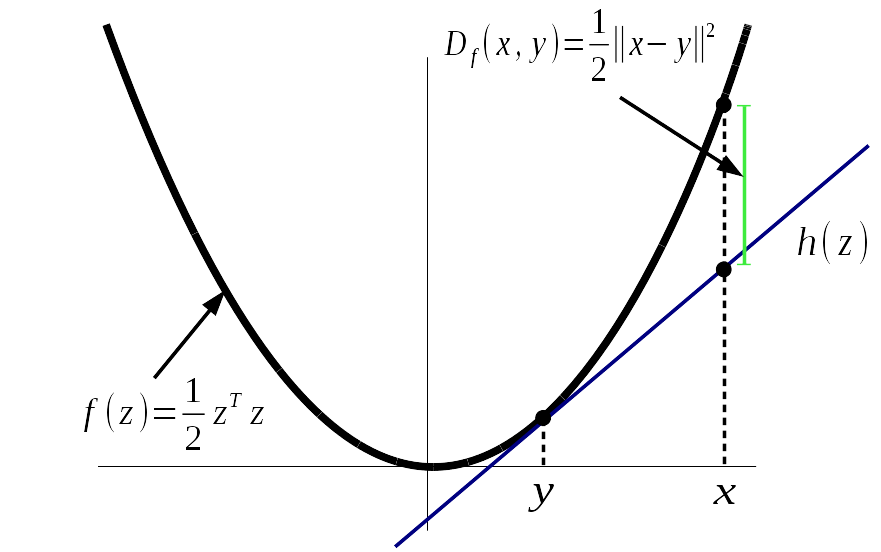
\includegraphics[width=0.6\columnwidth]{Figures/bregman_projection}
\caption{Geometry of the Bregman divergence with the seed function $f(z)=\frac{1}{2}z^\intercal z$. $h(z)$ is a hyperplane tangent to $f(z)$ at $y$. While it accurately represent $f(y)$, it underestimate $f(x)$. The Bregman divergence measures how much the representation of $f(x)$ on $h(z)$ \emph{diverges} from $f(x)$ (in green).}
\label{fig:bregman-projection}
\end{figure}
\iflatexml\else } \fi

\iflatexml\else \changes{ \fi
The scalar divergence can be directly adapted to SPD matrices as:
\begin{equation}
\divB{f}(\P_1,\P_2) = \varphi(\P_1) - \varphi(\P_2) - \varphi'(\P_2)(\P_1 - \P_2),
\end{equation}
where the seed function $f$ is combined with a function $g: \GenMa \rightarrow \Re^\dc$ that maps an SPD matrix to a vector containing its eigenvalues: $\varphi = f \circ \lambda$.\\
Or, $\lambda$ can be the trace function, $\lambda: \GenMa \rightarrow \Re$ that maps an SPD matrix to its trace.
For convenience, $f \circ \lambda$ will be referred to as $f(X)$ or $f(\P)$. 
\iflatexml\else } \fi
\iflatexml\else \changes{ \fi
Depending on the seed function used, various divergences can be defined defined from the Bregman divergence.

%- Squared Norm -> Euclidean divergence = Frobenious Norm (Dhillon 2007)
\\ \\ \textbf{Euclidean divergence} \\
The Frobenius norm is also a Bregman divergence in disguise. 
It is obtained when the seed function  is the squared norm $f(x) = \frac{1}{2} \lVert x \rVert_2^2$ \cite{dhillon_matrix_2007}:
\begin{equation}
\divB{E}(\P_1, \P_2) = \lVert \P_1-\P_2 \rVert _F
\label{eq:div-eucl}
\end{equation}
The Euclidean mean of SPD matrices correspond to their arithmetic mean \eqref{eq:mean_arithmetic}.
%\begin{equation}
%\PmE = \frac{1}{\Nb}\sum_{\nb=1}^{\Nb} \P_\nb
%\label{eq:mean-eucl}
%\end{equation} 

%- Shannon Entropy -> KL div (Nilson 2009)
\\ \\ \textbf{Kullback-Leibler divergence} \\
Using the \emph{Shannon entropy} $f(x) = \sum_\nb x_\nb \log x_\nb$ yields the \emph{Kullback-Leibler} divergence \cite{nielsen_sided_2009}.
It is also known as the \emph{relative entropy} or \emph{discrimination information}. The Kullback-Leibler divergence of SPD matrices $\P_1, \P_2 \in \Ma$ is given by:
\begin{equation}
\divB{KL}(\P_1, \P_2) = \frac{1}{2} \log \frac{\det(\P_2)}{\det(\P_1)} + \tr(\P_2 \P_1) - \dc
\label{eq:div-kl}
\end{equation}
The mean of SPD matrices induced by the Kullback-Leibler divergence is calculated iteratively \cite{chebbi_means_2012}. 

%- logarithmic barrier function -> Log det divergence (Dhillon 2007)
\\ \\ \textbf{Log-det divergence} \\
Another function often used in Bregman divergences of symmetric matrices is the \emph{logarithmic barrier} \cite{chebbi_means_2012,dhillon_matrix_2007,cherian_efficient_2011,sra_positive_2016}
\[ f(x) = -log(x) \rightarrow f(\P) = -\log \det(\P) \] 
The corresponding divergence is called the \emph{log-det} divergence and is given by \cite{chebbi_means_2012}:
\begin{equation}
\divB{ld}(\P_1,\P_2) = \left\langle \P_1, \P_2^{-1} \right\rangle - \log \det(\P_1 \P_2^{-1})-\dc
\label{eq:div-log-det}
\end{equation}
\iflatexml\else } \fi
\iflatexml\else \changes{ \fi
The asymmetry of divergences result in the concept of right- and left-sided mean:
\[ \divB{f}(\P_1,\P_2) \neq \divB{f}(\P_2,\P_1) \Rightarrow \argmin_{\P \in \Ma} \sum_{\nb=1}^{\Nb} \dist^2(\P_\nb,\P) \neq \argmin_{\P \in \Ma} \sum_{\nb=1}^{\Nb} \dist^2(\P, \P_\nb) \]
It is usually sufficient to consider a single sided divergence. 
In this work right-sided divergence and mean are used.
In some cases however, the asymmetry can be undesirable. This has led to the symmetrization of some Bregman divergences.
Often the symmetrization consist in an averaging of left- and right-sided divergence [todo: reference].

\\ \\ \textbf{S-divergence}\\
An example of a symmetric divergence is the S-divergence. 
It is obtained from the \emph{Jensen-Shannon} divergence which is a symmetrized Bregman divergence:
\begin{equation}
\begin{split}
\divB{J-S}(\P_1, \P_2) & = \frac{1}{2} \left( \divB{f}(\P_1,\frac{\P_1+\P_2}{2}) + \divB{f}(\frac{\P_1+\P_2}{2},\P_2) \right) \\
 & = \frac{1}{2} \left( \tr f(\P_1) + \tr f(\P_2) \right) - \tr f(\frac{\P_1+\P_2}{2})
\end{split} 
\label{eq:div-js}
\end{equation}
The S-divergence is obtained by using the logarithmic barrier function for the positive definite cone $f(\P)=-\log \det(\P)$ as seed in $\divB{S-J}$ \cite{sra_positive_2016}:
\begin{equation}
\divB{S}(\P_1,\P_2) = \log \det(\frac{\P_1+\P_2}{2}) - \frac{1}{2}\log \det(\P_1 \P_2)
\label{eq:div-s}
\end{equation}  
Despite its symmetry, S-Divergence is not a metric. It does not satisfy the triangular inequality criterion. 
However, its square root has been shown to be a distance \cite{sra_positive_2016}.
\iflatexml\else } \fi

\iflatexml\else \changes{ \fi
Other symmetric divergences can be obtained in the same fashion; for instance the \emph{Jeffreys divergence} which is a symmetrized Kullback-Leibler divergence: $\divB{J}(\P_1, \P_2) = \divB{KL}(\P_1, \P_2) + \divB{KL}(\P_2, \P_1)$ \cite{sra_positive_2016}.
\iflatexml\else } \fi

\iflatexml\else \changes{ \fi
Another family of divergence is defined when the right- and left-sided divergence are mixed in a weighted manner.
One such family is the \emph{$\alpha$-divergence} \cite{nielsen_clustering_2014}.
\\ \\ \textbf{Log-det $\alpha$-divergence}\\
In this work, the $\alpha$-divergence used is defined by \cite{chebbi_means_2012}:
\begin{equation}
\divB{f}^\alpha(\P_1,\P_2) = \frac{4}{1-\alpha^2}\left[ \frac{1-\alpha}{2} f(\P_1) + \frac{1+\alpha}{2}f(\P_2) - f \left( \frac{1-\alpha}{2}\P_1 + \frac{1+\alpha}{2}\P_2 \right) \right], \alpha^2 \neq 1
\label{eq:div-alpha}
\end{equation}
$\divB{f}^\alpha$ can be expressed in terms of Bregman divergence as:
\begin{equation}
\divB{f}^\alpha = \frac{4}{1-\alpha^2}\left[\frac{1-\alpha}{2}\divB{f}\left(\P_1, \frac{1-\alpha}{2}\P_1+\frac{1+\alpha}{2}\P_2\right) + \frac{1+\alpha}{2}\divB{f}\left(\P_2, \frac{1-\alpha}{2}\P_1 + \frac{1+\alpha}{2} \P_2 \right)\right], \alpha^2 \neq 1
\label{eq:div-alpha2}
\end{equation}
$\alpha$-divergences at $\alpha = \pm 1$ are obtained through the limit values $\lim_{\alpha \rightarrow \pm 1}\divB{f}^\alpha$.\\
Using the logarithmic-barrier function yields:
\begin{equation}
\begin{split}
\divB{LD}^\alpha(\P_1,\P_2) &= \frac{4}{1-\alpha^2}\log \det \left(\frac{1-\alpha}{2}\left(\P_1 \P_2^{-1}\right)^{\frac{1+\alpha}{2}}+\frac{1+\alpha}{2}\left(\P_2 \P_1^{-1}\right)^{\frac{1-\alpha}{2}}\right), \quad -1 < \alpha < 1 \\
\divB{LD}^{1}(\P_1,\P_2) &= \tr \left( \P_2^{-1}\P_1-\eye \right) - \log \det \left(\P_2^{-1}\P_1 \right)\\
\divB{LD}^{-1}(\P_1,\P_2) &= \tr \left(\P_1^{-1}\P_2-\eye \right) - \log \det \left(\P_1^{-1}\P_2 \right) .
\end{split}
\label{eq:div-log-det-alpha}
\end{equation}   
$\divB{LD}^{1}$ and $\divB{LD}^{-1}$ are right- and left-sided Bregman divergences respectively.
At $\alpha=0$, the log-det $\alpha$ divergence yields a symmetric divergence corresponding to the \emph{Bhattacharrya} divergence \cite{chebbi_means_2012,sra_positive_2016}. 
\iflatexml\else } \fi

%\subsubsection{log-det alpha divergence}
%\subsubsection{Kullback Leibler divergence}
%\subsubsection{Bhattacharyya}
%\subsubsection{S-divergence}

\subsubsection{Wasserstein}

\begin{table}[h]
  \centering
  \begin{tabular}{ l | c | c | c |}
    \cline{2-4}
    & Distance/Divergence & Mean & References \rule[-5pt]{0pt}{18pt} \\ \hline
    \multicolumn{1}{|l|}{Euclidean} & $\distF(\P_1, \P_2) = \lVert \P_1-\P_2 \rVert _F$ & $\PmE = \frac{1}{\Nb}\sum_{\nb=1}^{\Nb} \P_\nb$ & \rule[-5pt]{0pt}{18pt} \\   
		 \multicolumn{1}{|l|}{Log-Euclidean} & $\distLE(\P_1, \P_2) = \lVert \log(\P_1)-\log(\P_2) \rVert_F$ & $\PmLE = \exp \left(\sum_{\nb=1}^{\Nb} \log(\P_\nb) \right) $ & \cite{arsigny_geometric_2007} 
		\rule[-5pt]{0pt}{18pt} \\    
     \multicolumn{1}{|l|}{Affine-invariant} & $\distAIRM(\P_1, \P_2) = \lVert \log(\P_1^{-1}\P_2) \rVert_F$ & Algorithm 3 in \cite{fletcher_principal_2004}  & \cite{moakher_differential_2005,letcher_principal_2004} 
		\rule[-5pt]{0pt}{18pt} \\	
	\multicolumn{1}{|l|}{Kullback-Leibler} & $\divB{KL}(\P_1, \P_2) = \frac{1}{2} \log \frac{\det(\P_2)}{\det(\P_1)} + \tr(\P_2 \P_1) - \dc$ & Algorithm 1 in \cite{chebbi_means_2012} & \cite{chebbi_means_2012,kang_composite_2009} \rule[-5pt]{0pt}{18pt} \\
	\multicolumn{1}{|l|}{S-divergence} & $\divB{S}(\P_1,\P_2) = \log \det(\frac{\P_1+\P_2}{2}) - \frac{1}{2}\log \det(\P_1 \P_2)$ &  Eq. (17-20) in \cite{cherian_efficient_2011} & \cite{sra_positive_2016,cherian_efficient_2011} \rule[-5pt]{0pt}{18pt} \\
    \multicolumn{1}{|l|}{$\alpha$-divergence} & $\divB{LD}^\alpha (\P_1, \P_2)$ from Eq.~\eqref{eq:div-log-det-alpha} & Algorithm 1 in \cite{chebbi_means_2012} & \cite{chebbi_means_2012} \rule[-5pt]{0pt}{18pt} \\ 
    \multicolumn{1}{|l|}{Bhattacharyya} & $\divB{B}(\P_1, \P_2)=\left( \log \frac{ \det \frac{1}{2} (\P_1+\P_2)}{(\det (\P_1)\det(\P_2))^{1/2}} \right)^{1/2}$ & Algorithm 1 in \cite{chebbi_means_2012} & \cite{nielsen_matrix_2012,chebbi_means_2012} \rule[-5pt]{0pt}{18pt} \\ 
    \multicolumn{1}{|l|}{Wasserstein} &  &  &  \rule[-5pt]{0pt}{18pt} \\ \hline
  \end{tabular}
  \caption{Distances, divergences and means considered in the experimental study.}
  \label{tab:dist}
\end{table}
\subsection{Minimum Distance to Mean classifier for SSVEP}
\label{subsec:mdm}
\iflatexml\else \changes{ \fi 
The considered classifier is described in section \ref{subsec:fund_class}. 
\iflatexml\else } \fi
It is given the name \emph{Minimum Distance to Mean} or MDM, and was inspired from~\cite{barachant_multiclass_2012} where it is limited to Riemannian mean.
%The considered classifier is referred to as Minimum Distance to Mean (MDM), and is inspired from~\cite{barachant_multiclass_2012} where it is limited to Riemannian mean. 
Covariance matrices of EEG trials are classified based on their distance to the centers of the classes (i.e. means or centroids).
To embed frequency information in the covariance matrices, we use a construction of matrices proposed in~\cite{congedo_new_2013}.
%In a SSVEP experiment with $\dF$ stimulus blinking at $\dF$ different frequencies, 
Let $\X \in \Re^{\dc\times\dt}$ be an EEG trial measured on $\dc$ channels and $\dt$ samples in a SSVEP experiment with $\dF$ stimulus blinking at different frequencies.  
The covariance matrices are estimated from a modified version of the input signal $\X$: %as explained in~\cite{congedo_new_2013}
%%Let $X \in \Re^{p \times n}$ be the recorded data with $p$ the number of channels, and $n$ the number of sample per trial. 
%%The extended data are defined as:
%Let consider an experimental SSVEP setup with $\dF$ stimulus blinking at $\dF$ different frequencies. 
%It is a multiclass classification with $\dK=\dF+1$ classes: one class per stimulus and one resting state class.
%The covariance matrices are estimated from a modified version of the input signal $\X$: %as explained in~\cite{congedo_new_2013}
%Let $X \in \Re^{p \times n}$ be the recorded data with $p$ the number of channels, and $n$ the number of sample per trial. 
%The extended data are defined as:
\begin{equation}
	\X \in \Re^{\dc \times \dt} \rightarrow 	
	\begin{bmatrix}
		X_{\text{freq}_1}\\ \vdots \\ X_{\text{freq}_{\dF}} \\
	\end{bmatrix}
	\in \Re^{\dF\dc \times \dt} \ ,
	\label{eq:ext_data}
\end{equation}
where $X_{\text{freq}_\df}$ is the input signal $\X$ band-pass filtered around frequency $\text{freq}_\df$, $\df=1, \ldots, \dF$. Henceforth, all EEG signals will be considered as filtered and modified by Eq.~\eqref{eq:ext_data}.
The associated covariance matrix $\P \in \Re^{\dF\dc \times \dF\dc}$ is estimated using the Sch\"{a}fer skrinkage estimator \cite{schafer_shrinkage_2005}.

For SSVEP classification, $\dK = \dF + 1$ classes are considered: one class for each target frequency, and one for the resting state.
As described in Algorithm~\ref{alg:mdm}, from $\dT$ labelled training trials $ \left\{ \X_{\ti} \right\}_{\ti=1}^{\dT}$ recorded per subject, $\dK$ centers of classes $\Pm^{(\ci)}$ are estimated (step~\ref{op:class_center}). 
In this step, outliers matrices are removed to have a reliable mean estimation \cite{barachant2013riemannian}.
A new unlabeled test trial $\Y$ is predicted to belong to the class whose mean $\Pm^{(\ci)}$ is the closest to the trial covariance matrix, w.r.t. one of the distances from Table~\ref{tab:dist} (step~\ref{op:decision}).

\begin{algorithm}
\caption{Minimum Distance to Mean Classifier}
\label{alg:mdm}
	Inputs: $\X_{\ti} \in \Re^{\dF \dc\times\dt}$, for $\ti = 1, \ldots, \dT$, a set of labelled EEG trials. \\
	Inputs: $\setindex(\ci)$, a set of indices of trials belonging to class $\ci$. \\
	Input: $\Y \in \Re^{\dF \dc\times\dt}$, an unlabeled test EEG trial. \\
	Output: $\clout$, the predicted label of $\Y$.
	\begin{algorithmic}[1]
	\State Compute covariance matrices $\P_{\ti}$ of $\X_\ti$ 
	\State \textbf{for} $\ci$ = 1 \textbf{to} $\dK$ \textbf{do}
	\State \quad Compute center of class : $\Pm^{(\ci)}=\Rm(\P_{\ti}:\ti \in \setindex(\ci))$
	\label{op:class_center}
	\State \textbf{end}
	\State Compute covariance matrix $\P$ of $\Y$, and classify it : $\clout = \arg \min_{\ci} \dist(\P, \Pm^{(\ci)})$
	\label{op:decision}
	\State \textbf{return} $\clout$
	\end{algorithmic}
\end{algorithm}

%%%%%%%%%%%%%%%%%%%%%%%%%%%%%%%%%%%%%%%%%%%%%%%%%%%%%%%%%%%%%%%%%%%%%%%%%%%%%%%%


